\documentclass{article}
\usepackage[utf8]{inputenc}
\usepackage[margin=1in]{geometry}
\usepackage[titletoc,title]{appendix}
\usepackage{amsmath,amsfonts,amssymb,mathtools}
\usepackage{graphicx,float}
\usepackage[ruled,vlined]{algorithm2e}
\usepackage{algorithmic}
\usepackage{biblatex}
\usepackage{tikz}
\usepackage{matlab-prettifier}
\usepackage{listings}
\usepackage{xcolor}
\usepackage{hyperref}
\usepackage{caption}
\usepackage{subfig}
\addbibresource{references.bib}

\newcommand{\hmwkTitle}{Homework 2}
\newcommand{\hmwkDueDate}{February 7, 2020}
\newcommand{\hmwkClass}{Computational Methods for Data Analysis}
\newcommand{\hmwkClassNum}{AMATH 582}
\newcommand{\hmwkClassInstructor}{Professor J. Nathan Kutz}
\newcommand{\hmwkAuthorName}{\textbf{Chandan Sharma Subedi}}
\newcommand{\hmwkClassSection}{Section A}

%
% Title Page
%

\title{
    \vspace{2in}
    \textmd{\textbf{\hmwkClass}}\\
    \vspace{0.3in}\textmd{\textbf{\hmwkTitle}}\\
    \normalsize\vspace{0.1in}\small{Due\ on\ \hmwkDueDate\ at 11:00pm}\\
    \vspace{0.1in}\large{\textit{\hmwkClassInstructor}} \\
    \vspace{0.1in}\large{{\hmwkClassSection}} \\
    \vspace{2.5in}
}

\author{\hmwkAuthorName}
\date{}

\begin{document}

\maketitle
\pagebreak

% Abstract
\begin{abstract}
Frequency analysis of a signal through Fourier Transform is a very useful tool to analyze stationary signal. However, when the frequency signature of a signal changes over time, frequency analysis does not give adequate information to analyze the signal. The paper discusses a novel time-frequency analysis based on Gabor Transform that extends the idea of Fourier Tranform to produce a spectrogram of a signal. The spectrogram is later used to identify notes played on the piano and recorder recordings of the song \textit{"Mary had a little lamb."}.
\end{abstract}

% Introduction and Overview
\section{Introduction and Overview}
Fourier Transform was an influential idea that revolutionlized radar technology in $1940$s. A Fourier Transform of a signal gives the frequency content of the signal. However, when frequencies in the signal change with time, Fourier Transform becomes less useful. It does not tell us at what point each frequency is active. The figure \ref{fig:nonstationary} shows that even though Fourier Transform gives all frequencies in the signal, it is not clear when $10$ Hz frequency is active.

Gabor in $1946$ came up with an idea of using a sliding window that would allow us to assume the signal under the window as stationary. Through sliding window, the time information of the frequency spectrum is captured that gives us a $2$D data with good time and frequency resolution (as shown in figure \ref{fig:resolution}). Section \ref{Introduction} gives a detailed theoretical background on Gabor Transform and sliding windows. Section \ref{Algorithm} and \ref{Result} discuss the implementation of Gabor Transform to analyze music recording and results of the analysis.

\begin{figure}[!b]
  \centering
    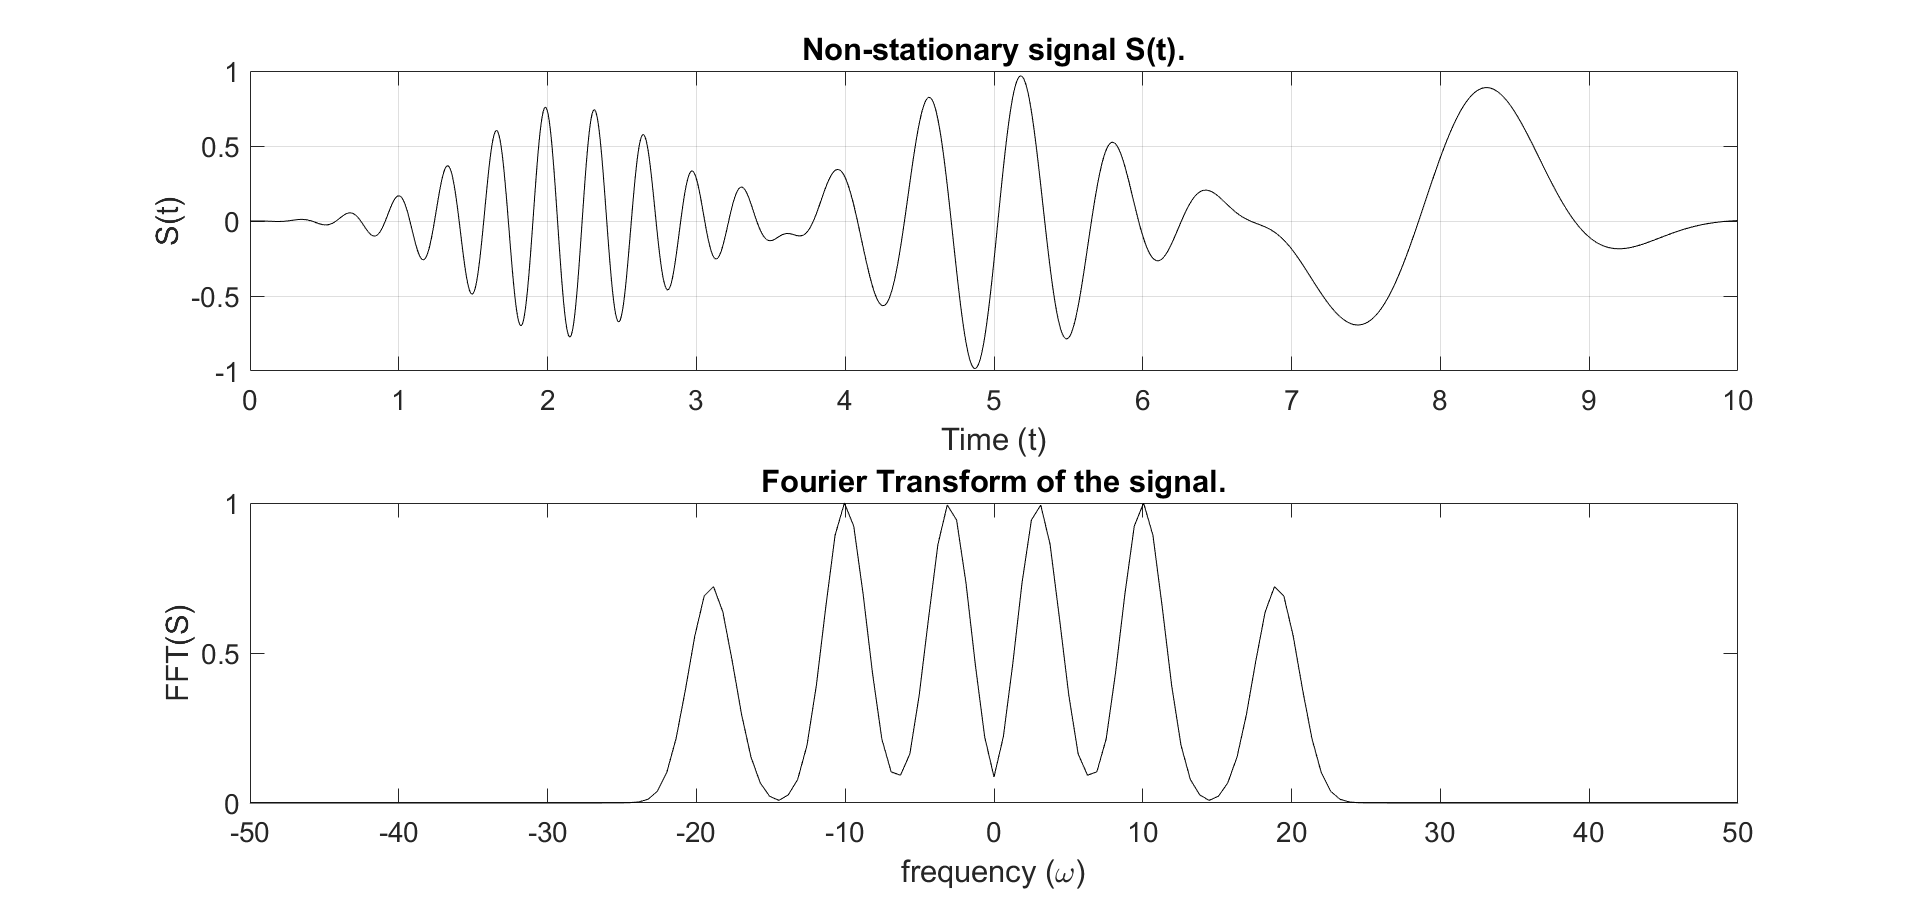
\includegraphics[scale=0.28]{./Figures/nonstationary.png}
    \caption{The figure shows a non-stationary signal and its fast fourier transform.}
  \label{fig:nonstationary}
\end{figure}

\begin{figure}[!b]
\centering
\subfloat[Time Analysis]{
\begin{tabular}{|c|c|c|c|c|c|c|}
 \hline
 &  &  &  &  & & \\ 
 &  &  &  &  & & \\ 
 &  &  &  &  &  & \\ 
 &  &  &  &  &  & \\ 
 &  &  &  &  &  & \\ 
 &  &  &  &  &  & \\ 
 \hline
\end{tabular}}
\quad \quad 
\subfloat[Freq. Analysis]{
\begin{tabular}{ |c c c c c c c|} 
 \hline
 &  &  &  &  &  & \\
\hline 
 &  &  &  &  &  & \\ 
\hline
 &  &  &  &  &  & \\ 
\hline
 &  &  &  &  &  & \\ 
\hline
 &  &  &  &  &  & \\ 
\hline
 &  &  &  &  &  & \\ 
 \hline
\end{tabular}}
\quad \quad 
\subfloat[Gabor Transform]{
\begin{tabular}{ |c| c| c| c| c| c| c|} 
 \hline
 &  &  &  &  &  & \\
\hline 
 &  &  &  &  &  & \\ 
\hline
 &  &  &  &  &  & \\ 
\hline
 &  &  &  &  &  & \\ 
\hline
 &  &  &  &  &  & \\ 
\hline
 &  &  &  &  &  & \\ 
 \hline
\end{tabular}}
\caption{Time analysis gives a perfect resolution on when each frequencies are active, but no information about what those frequencies are. Frequency analysis gives perfect resolution on what all the frequencies are in the signal, but no information on when those frequencies are active. Time-Frequency analyis through Gabor Transform gives a good resolution (not perfect) on both time and frequency.}
\label{fig:resolution}
\end{figure}

\pagebreak
%  Theoretical Background
\section{Theoretical Background}\label{Introduction}
The discrete Gabor Tranform discretizes the signal through sliding window. Each window captures a piece of the signal, which is then fourier tranformed to gives its frequency spectrum. As we slide the window through the signal, we obtain a varying frequency spectrum. Combining these spectrums, we obtain a spectrogram that gives us a visual representation of how frequency spectrum varies over time in the signal.

Fourier Tranform of any periodic function in the interval $t \in (-\pi, \pi]$ is a complex valued function of frequency whose modulus is the amount of that frequency and argument is the phase of the sinusoid. Fourier transform is defined as
\begin{align*}
&F(k) = \int_{-\infty}^{\infty} f(t)e^{-ikt} dt 
\end{align*}

The Gabor Transform of the function $f(t)$ is defined as
\begin{align*}
&G_f(\tau, k) = \int_{-\infty}^{\infty} f(t)\overline{g}_a(\tau - t)e^{-ikt} dt 
\end{align*}
$g_a(\tau - t)$ is the sliding window obtained through the parameterization of function $g(t)$ over a scaling factor $a$ and a shifting factor $\tau$. The scaling factor $a$ determines the width of the window. In this assingment, following three sliding windows were examined:
\begin{align*}
&\textit{Gaussian: } \quad \quad \quad g_a(\tau - t) = e^{-a(\tau - t)^2} \\
&\textit{Mexican Hat:} \quad \quad g_a(\tau - t) = (1-a(\tau-t)^2)e^-{\Big(\frac{a(\tau-t)^2}{2}\Big)} \\
&\textit{Rectangle: } \quad \quad \quad
   g_a(\tau - t) = 
   \begin{cases}
     1 &\text{if $ (\tau + a/2) > t > (\tau - a/2)$} \\
     1/2 &\text{if $t = (\tau + a/2)$, $t = (\tau - a/2)$} \\
     0 &\text{otherwise}.
   \end{cases}
\end{align*}

All these functions have one similarity that allows them to be used as a sliding window. When we mulitply the signal with these functions, the signal that lies inside the window remains more or less unchanged, while the signal that lies outside the window approaches zero. Thus, these functions act as a window that isolates a part of a signal at a particular instance of time.

A spectrogram is generated by combining frequency spectrums obtained through the fourier tranform of windowed signals. Thus, it gives a visual representation of how frequency spectrum is changing over time. The resolution of spectrogram, obtained through Gabor Transform, depends strongly on the sliding window and its scaling and sliding parameters. This stems from the fact that the fundamental idea of Gabor Transform is to make some compromise on spectral resolution so as to gain some temporal resolution.

\begin{itemize}
\item Effect of scaling parameter on resolution of spectrogram: \\
If we choose a scaling parameter that gives a very narrow sliding window, then we will obtain a good temporal resolution but a poor spectral resolution. If $a$ is the width of the narrow sliding window, the smallest frequency it can identify is $1/a$. Thus, we will lose all low frequencies in the spectrum. On the other hand, if we choose a wide sliding window, then we will obtain a good spectral resolution but a poor temporal resolution. Thus, a scaling factor should be chosen that gives a good resolution for both time and frequency. 

\item Effect of sliding parameter on resolution of spectrogram: \\
\textbf{Undersampling:} If we slide window at time steps greater than half of the window width, then we are bound to completely miss a part of the signal. This will reduce both temporal and spectral resolution of the spectrogram. \\
\textbf{Oversampling:} If we slide window at very small time steps, it will slightly improve the temporal resolution but at a massive computational cost.
\end{itemize}


% Algorithm Implementation and Development
\section{Algorithm Implementation and Development}\label{Algorithm}
\subsection{Part I}
In Part I of the assignment, a portion of the Handel's Messiah was analyzed using Gabor Transform as the method of time-frequency analysis. Three different sliding window functions were used with varying scaling and sliding parameters. A MATLAB script was written to perform the following four computational procedures.

\begin{itemize}
\item \textbf{Generate a vector representing the data:} \\
The recording of the Handel's Messiah was tranformed into a column vector. The corresponding time vector was generated using the samping rate Fs.

\item \textbf{Construct the sliding window function:} \\
A sliding window was constructed by choosing a function (Gaussian, Mexican Hat or Rectangle) and parameterizing it with scaling parameter $a$ and sliding parameter $\tau$. A sliding time-step $\Delta t$ was chosen to find the sliding parameter at each step.

\item \textbf{Fast Fourier Transform of windowed signal:} \\
At each step of the slide, windowed signal was Fast Fourier transformed to generate the frequency spectrum. The spectrum was saved in an array for plotting.

\item \textbf{Generate Spectrogram:} \\
All frequency spectrums were plotted against time using \emph{pcolor} MATLAB function.
\end{itemize}
\subsection{Part II}
In Part II, we use Gabor filtering to reproduce the music score of the song \textit{"Mary had a little lamb"} recorded in piano and recorder. We use same steps as  in Part I to first generate spectrogram and then use music sheet to find the score.
\begin{itemize}
\item \textbf{Generate vectors representing the piano and recorder data:} 
\item \textbf{Construct the Gaussian sliding window function:} 
\item \textbf{Fast Fourier Transform of windowed signal:} 
\item \textbf{Generate Logarithmic spectrograms:} 
\item \textbf{Reproduce the music score in piano recording:} \\
The logarithmic spectrogram was zoomed near center freqeuncies and using the music sheet given in the assignment, the music score was reproduced.
\end{itemize}

% Computational Results
\section{Computational Results}\label{Result}
\subsection{Part I}
The audio considered for the analysis was a 8.9249 sec long audio recording of the Handel's Massiah, sampled at 8192 Hz. The audio was loaded from the MATLAB and a vector was created representing the audio. Using the sampling rate, the corresponding time vector was also calculated. A Gaussian sliding window was constructed with width (FWHM) $\approx 0.17$sec. The smallest frequency that a human ear can hear is $20$Hz. The wavelength of that signal will be $1/20 = 0.05$ sec. The window width guarantees that all frequencies audible to human ear will be detected during Gabor Transform. The figure \ref{fig:signal} shows
the process of filtering/windowing signal at each sliding step by the Gaussian window and finding its corresponding frequency spectrum through FFT. The spectrogram was generated by plotting all frequency spectrums against time using MATLAB \textit{pcolor} function. \\

The effect of scaling was explore by generating spectrogram for four different values of $a$ that changes the width of the window. 
The width of the Gaussian function was defined in terms of full width at half maximum (FWHM), which is the distance between half of maximum value. FWHM for our Gaussian function was derived as follow
\begin{align*}
\frac{1}{2} = e^{-a(\tau - t^*)^2} \Longrightarrow (\tau-t^*) = \sqrt{\frac{\ln2}{a}} \Longrightarrow \Delta = 2\sqrt{\frac{\ln2}{a}} \\
\end{align*}

The figure \ref{fig:scaling} shows how spectrogram resolution changes when the width of sliding window is changed. For large width, we saw a very good frequency resolution but a poor temporal resolution. However as window width was decreased, we saw improvement in temporal resolution but at the expense of spectral resolution. This makes sense, since smaller window will fail to capture low frequency signals, while increasing the time data. 
The figure \ref{fig:function} shows zoomed spectrograms produced by different window function with approximately the same width ($\approx 0.2$).  We can see that Mexican Hat function captures more frequency content and with less temporal resolution (observe right most part of the spectrogram) because it does not approach $0$ as fast as the other two functions. However Mexican Hat function trims more data inside its window because of its sharp peak. Spectrogram with Shannon function is close to one with Gaussian function. Because of sharp edges of Shannon function, we see discreteness in its spectrogram.

\begin{figure}[!t]
  \centering
    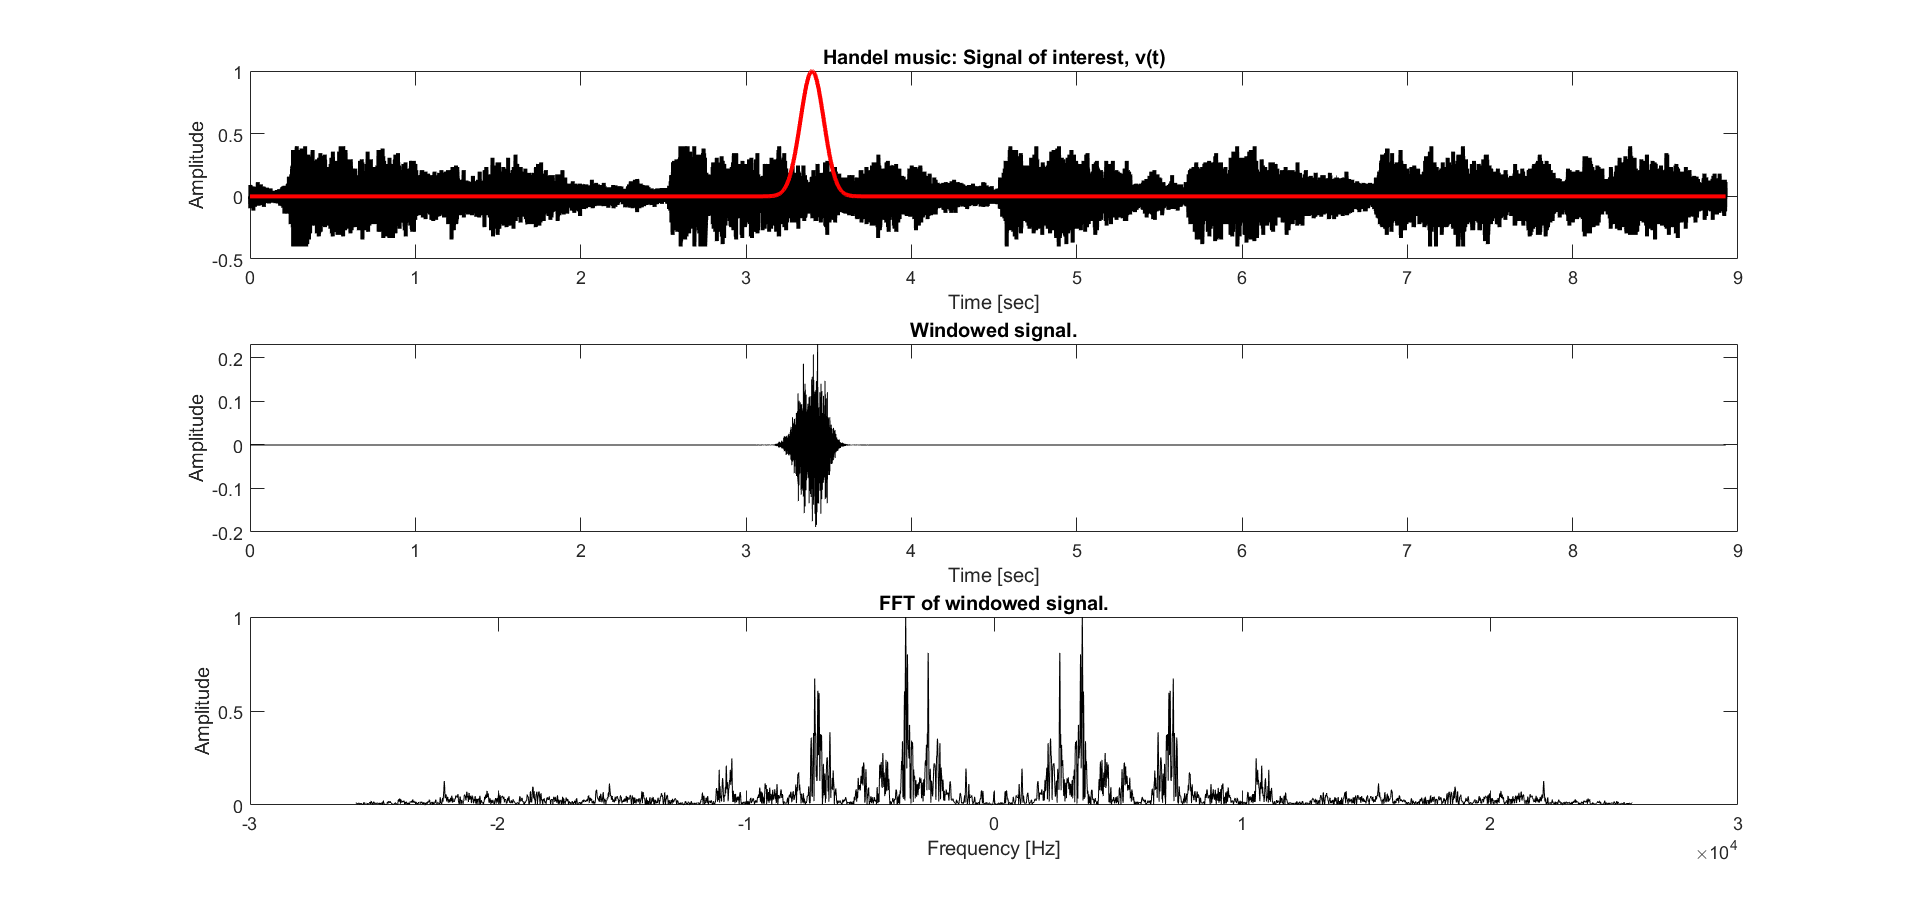
\includegraphics[scale=0.35]{./Figures/signal.png}
    \caption{The signal of interest is plotted along with the Gaussian sliding window (red). The corresponding filtered signal and its frequency spectrum is also plotted.}
  \label{fig:signal}
\end{figure}

\begin{figure}[!t]
\subfloat[Spectrogram using Gaussian filter of FWHM $\approx 3.7$]{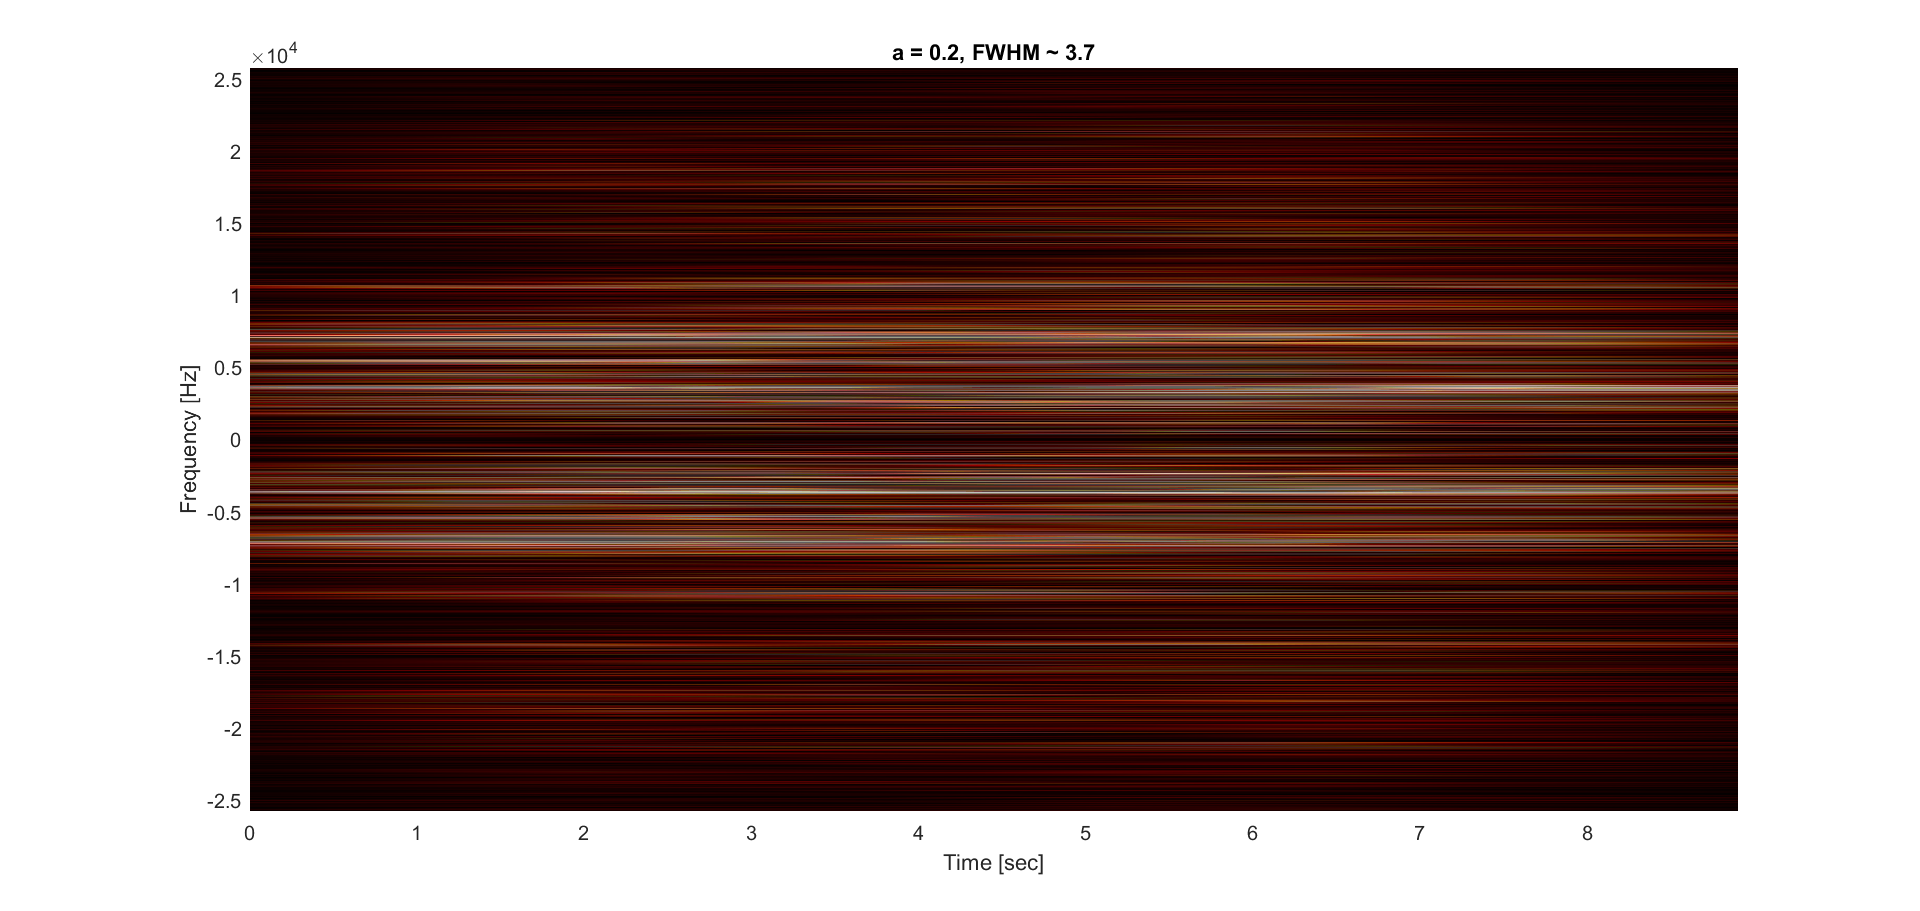
\includegraphics[width = 0.5\linewidth]{./Figures/widtha1}} 
\subfloat[Spectrogram using Gaussian filter of FWHM $\approx 1.7$]{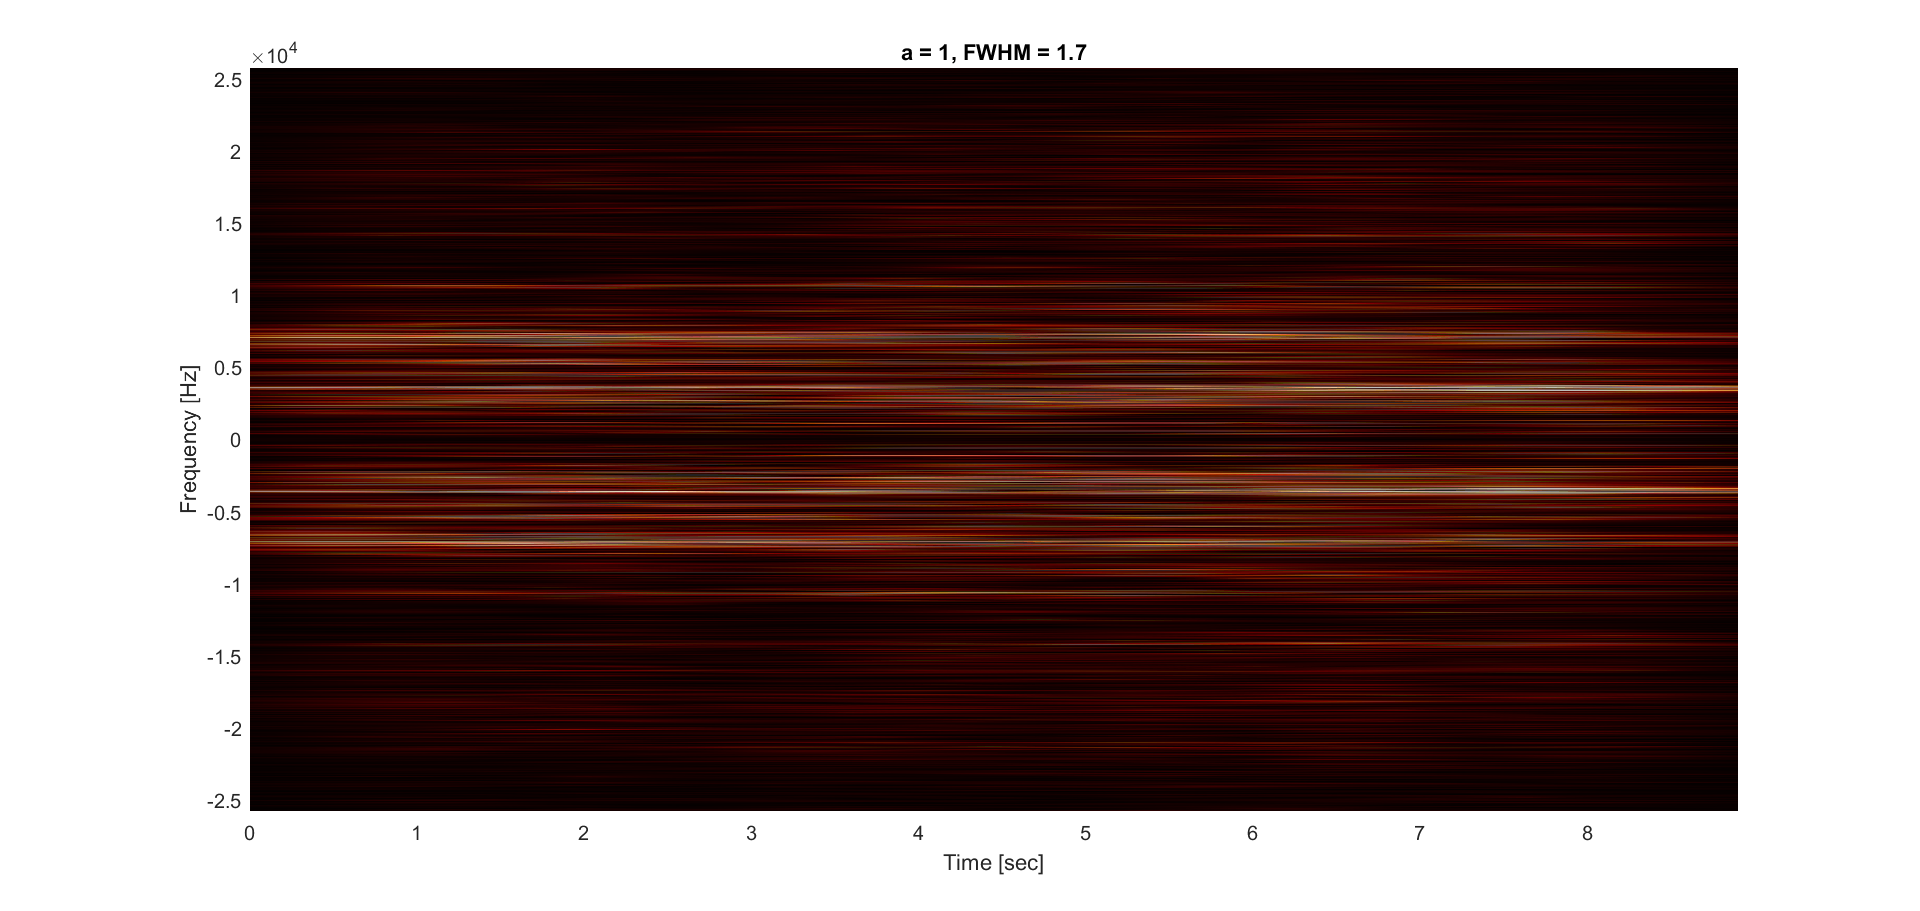
\includegraphics[width = 0.5\linewidth]{./Figures/widtha2}}\\
\subfloat[Spectrogram using Gaussian filter of FWHM $\approx 0.4$]{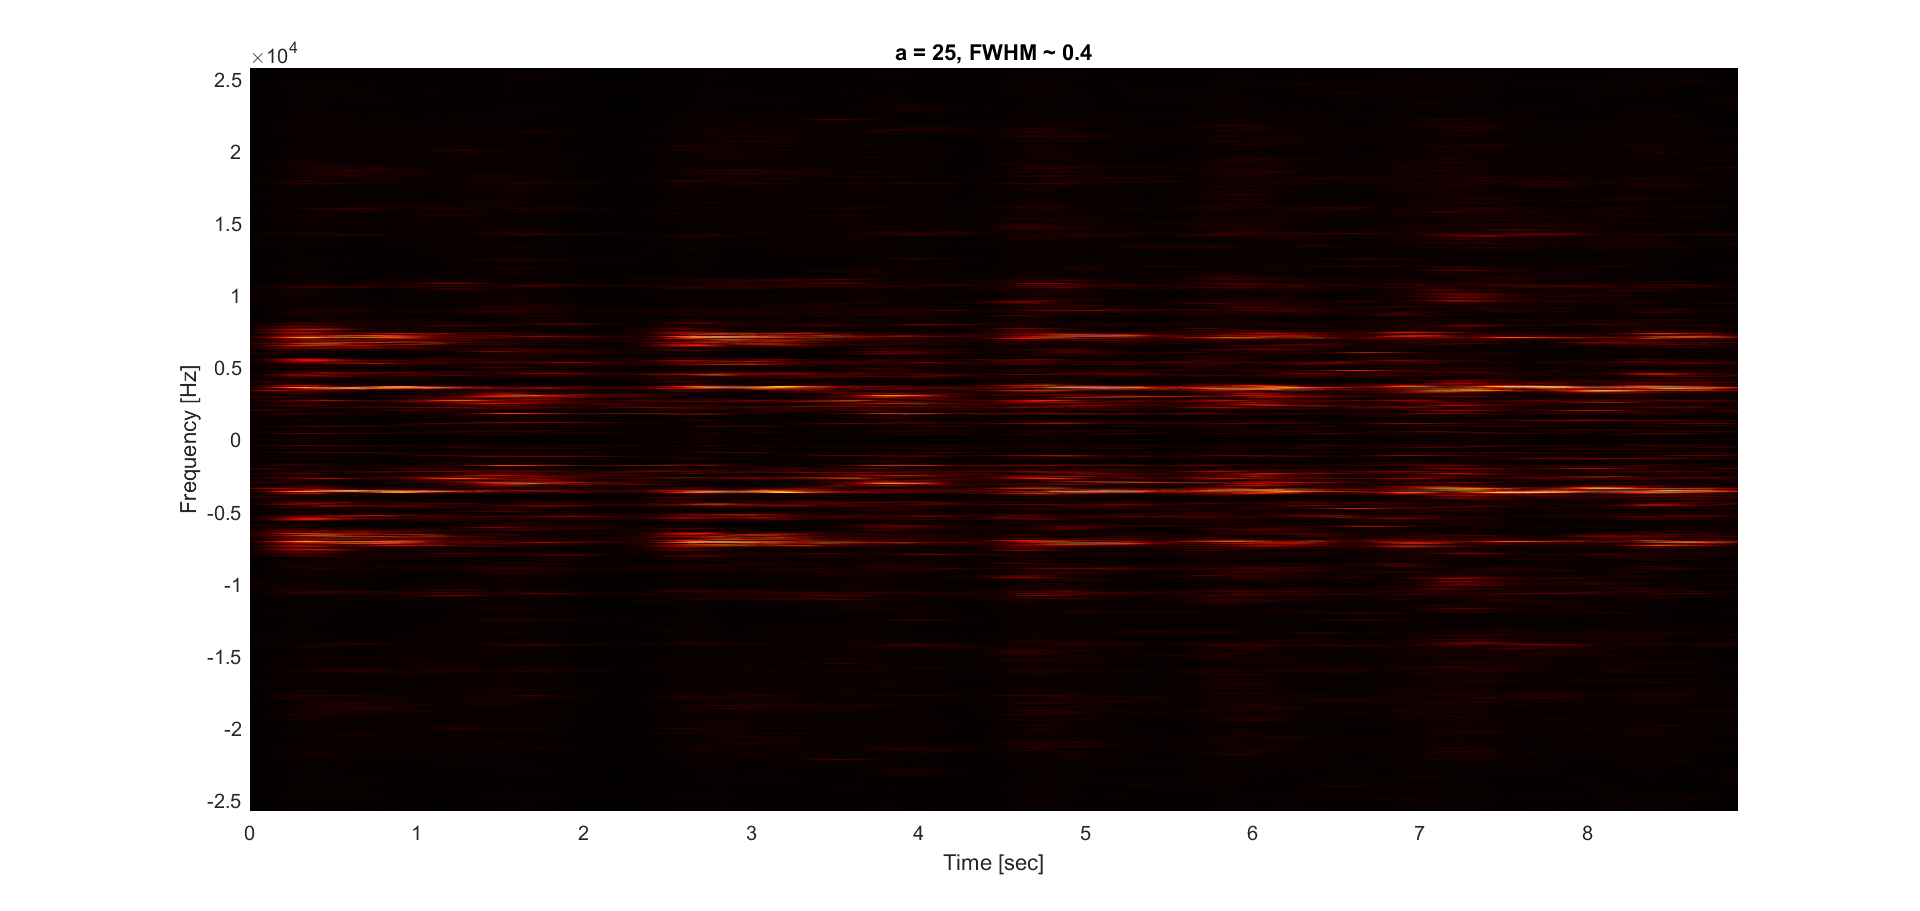
\includegraphics[width = 0.5\linewidth]{./Figures/widtha3}}
\subfloat[Spectrogram using Gaussian filter of FWHM $\approx 0.2$]{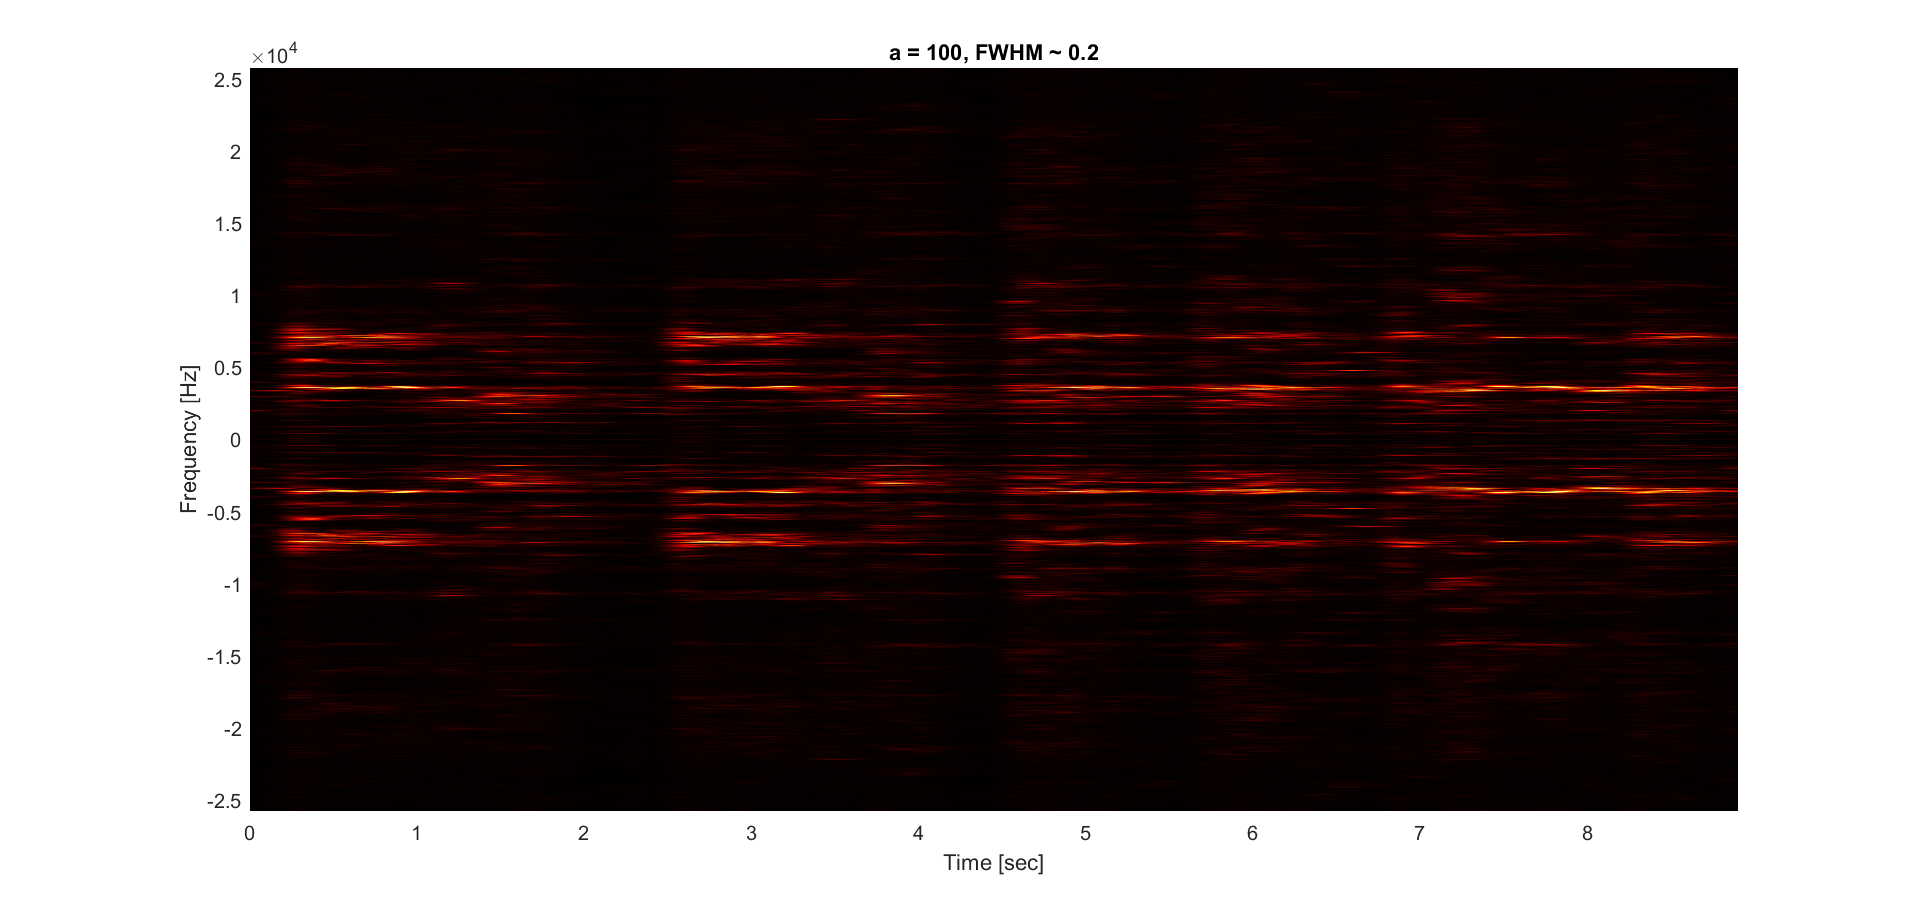
\includegraphics[width = 0.5\linewidth]{./Figures/widtha4}} 
\caption{Four spectrograms show the effect of scaling parameter $a$ on the spectral and temporal resolution. }
\label{fig:scaling}
\end{figure}

\begin{figure}[!h]
\subfloat[Shannon function.]{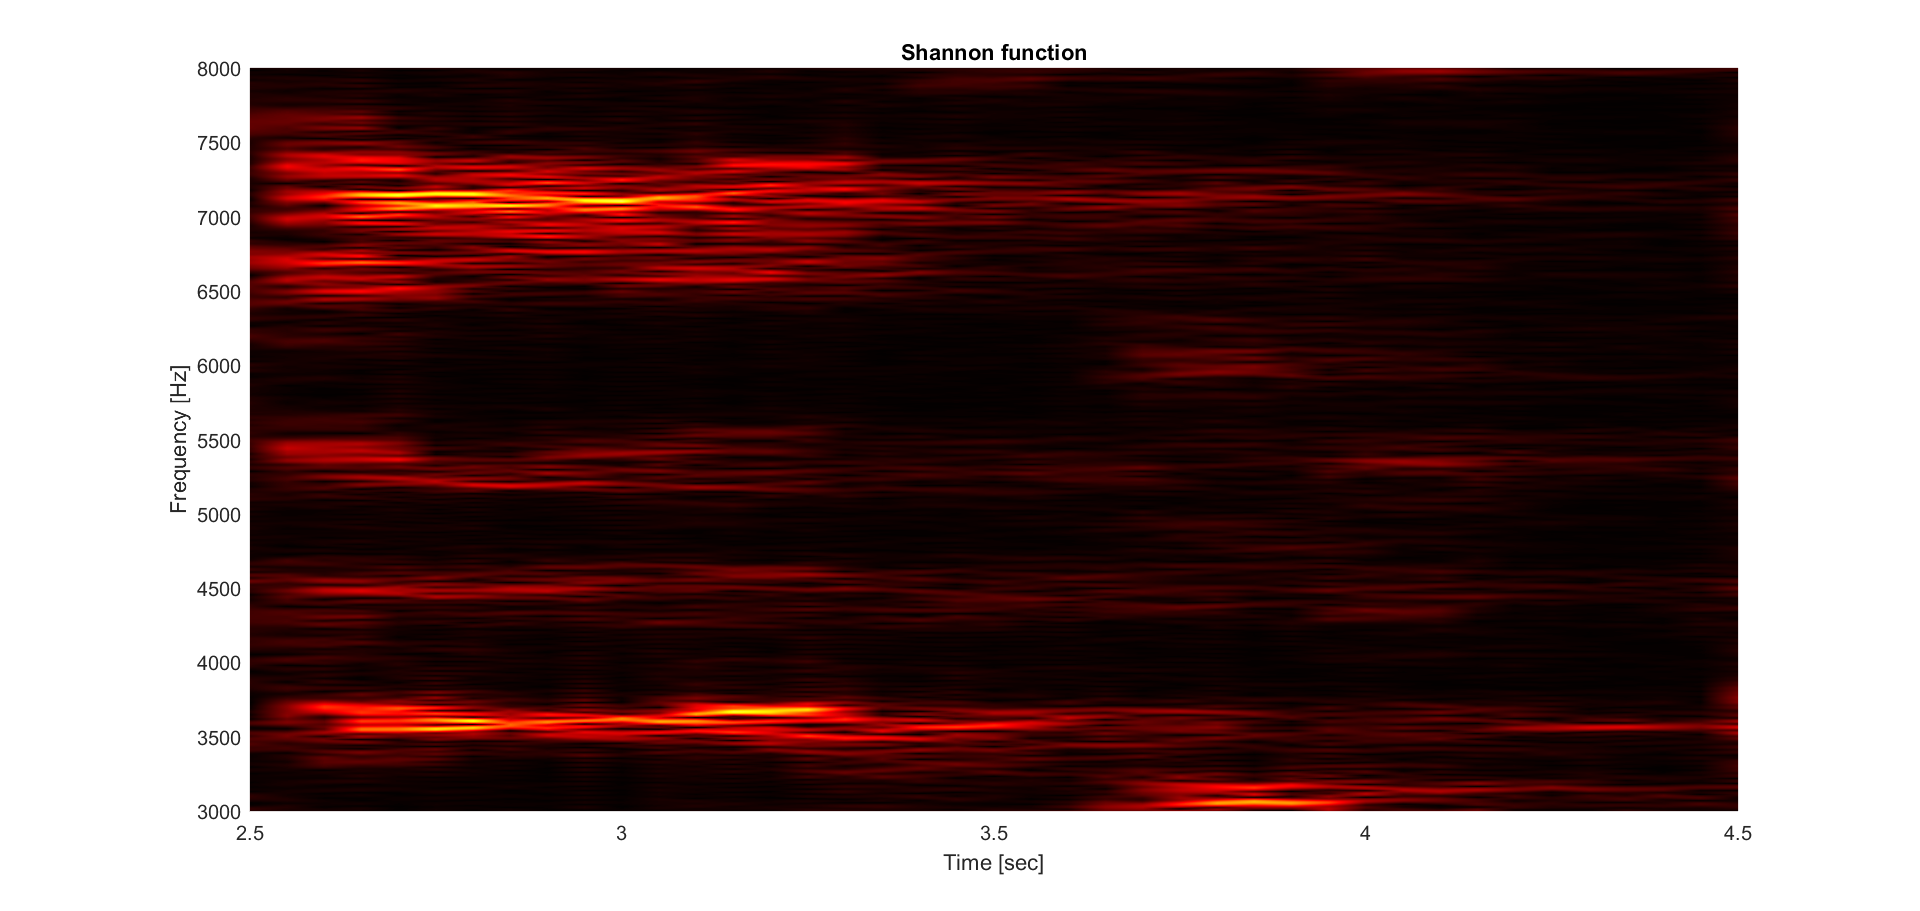
\includegraphics[width = 0.33\linewidth]{./Figures/shannon2}\hspace{0in}} 
\subfloat[Mexican Hat function. ]{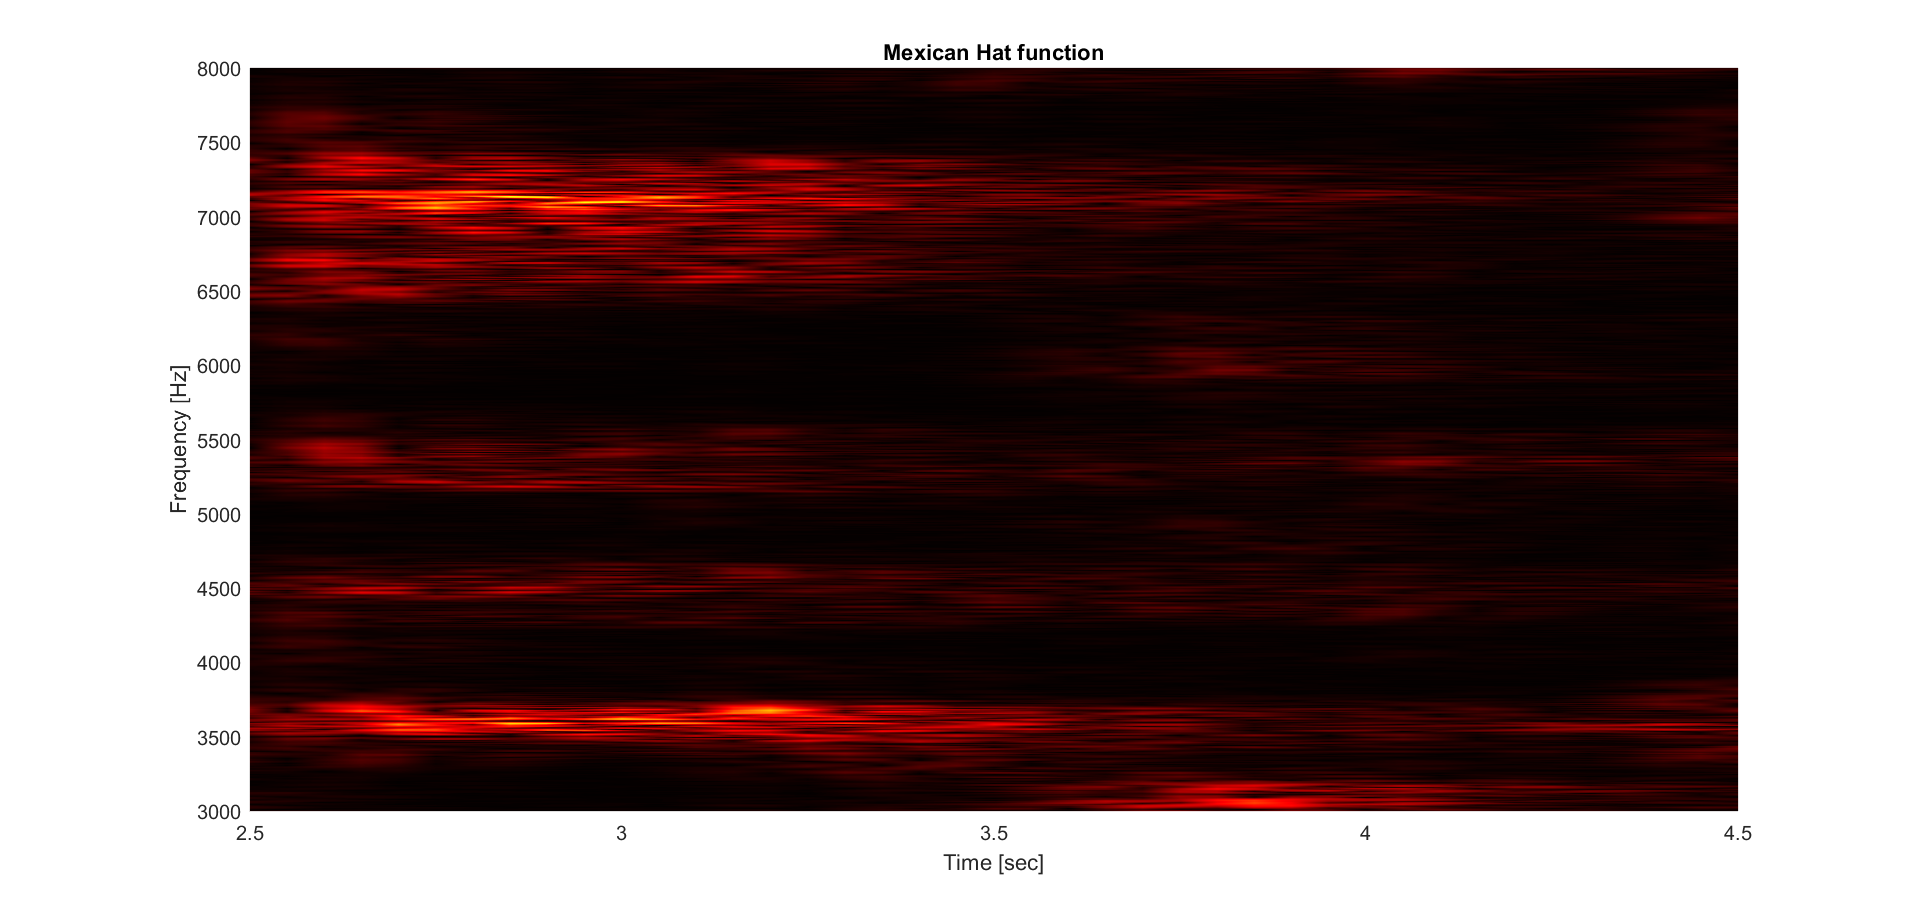
\includegraphics[width = 0.33\linewidth]{./Figures/Mexicanhat2}}
\subfloat[Gaussian function.]{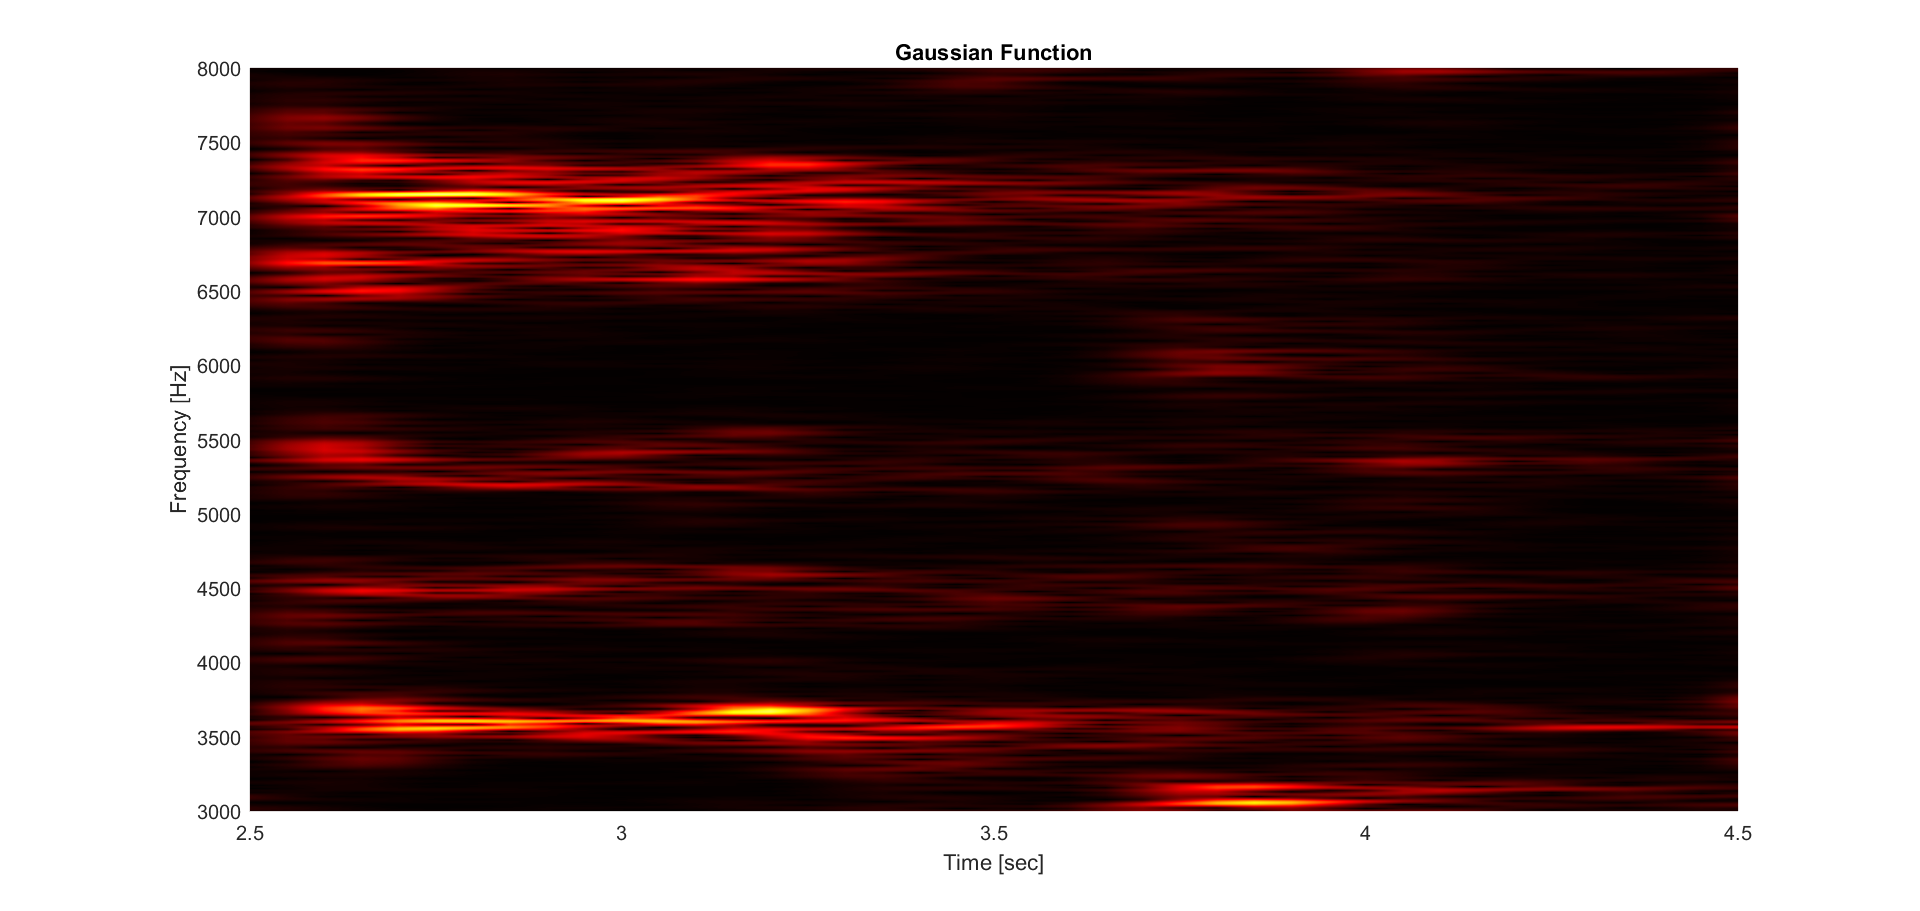
\includegraphics[width = 0.33\linewidth]{./Figures/Gaussian2}}
\caption{Three zoomed spectrograms shows the effect of sliding window function on the spectral and temporal resolution (for same window width). }
\label{fig:function}
\end{figure}

\begin{figure}[!h]
\subfloat[Undersampling with $\Delta \tau = 0.5$.]{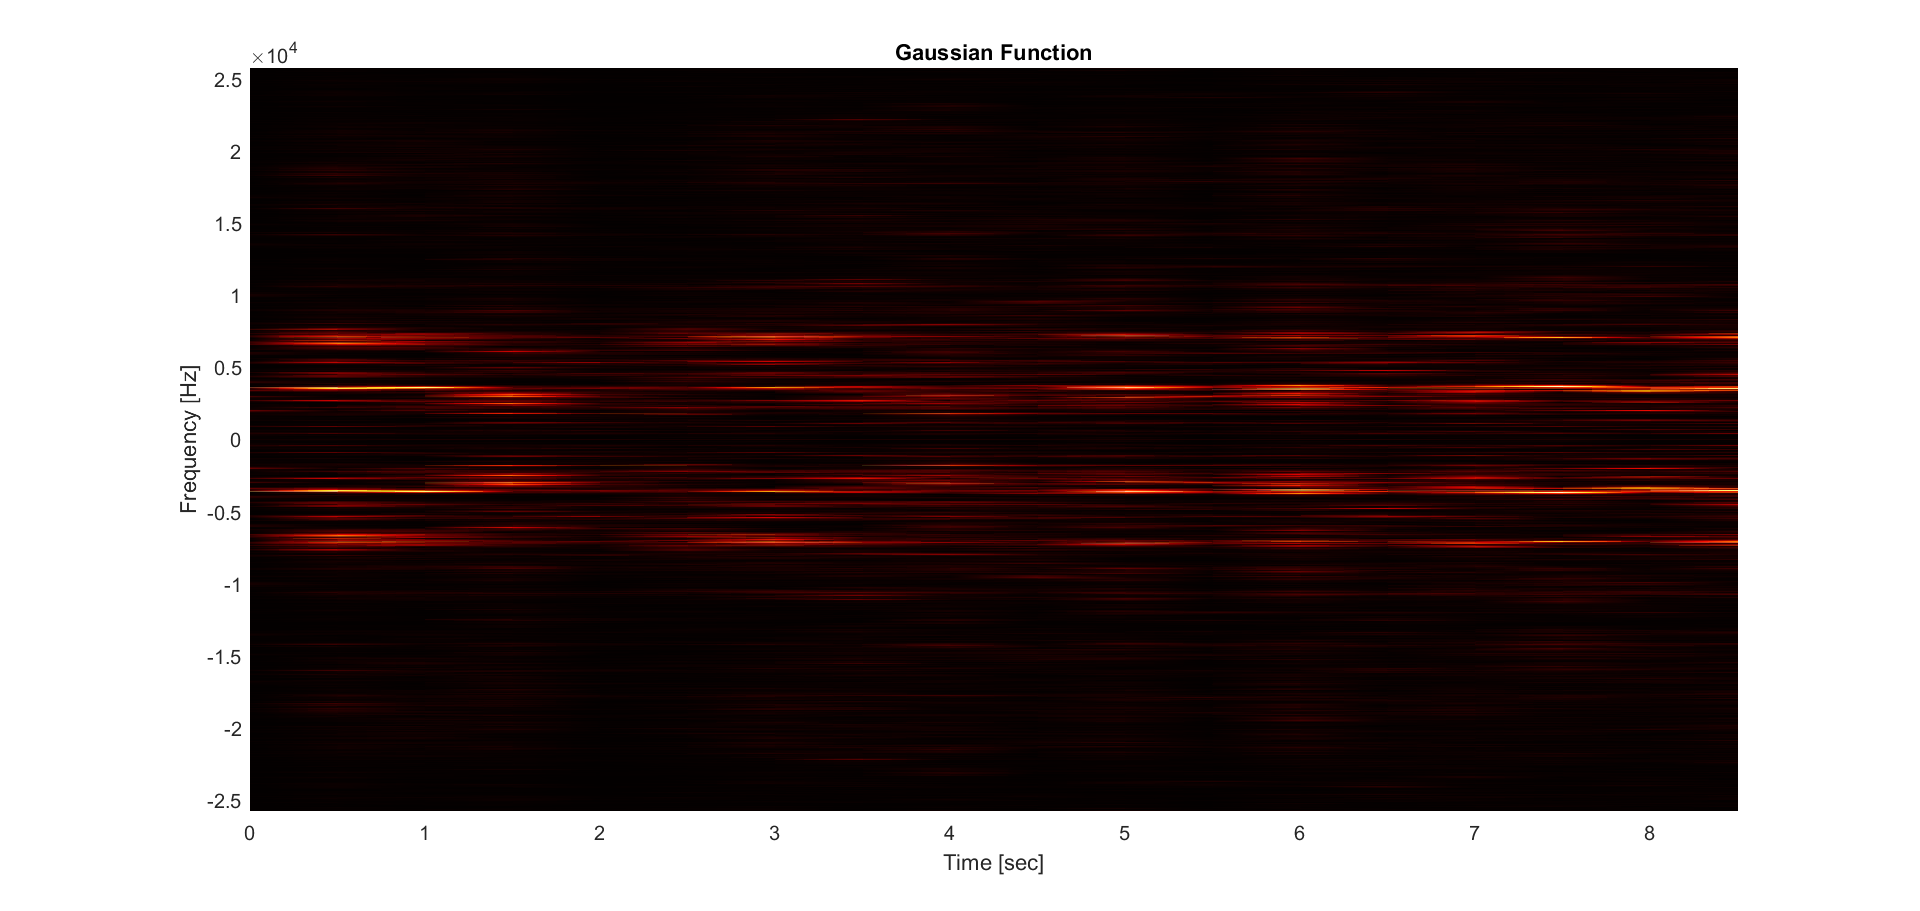
\includegraphics[width = 0.5\linewidth]{./Figures/undersample05}} 
\subfloat[Oversampling with $\Delta \tau = 0.01$.]{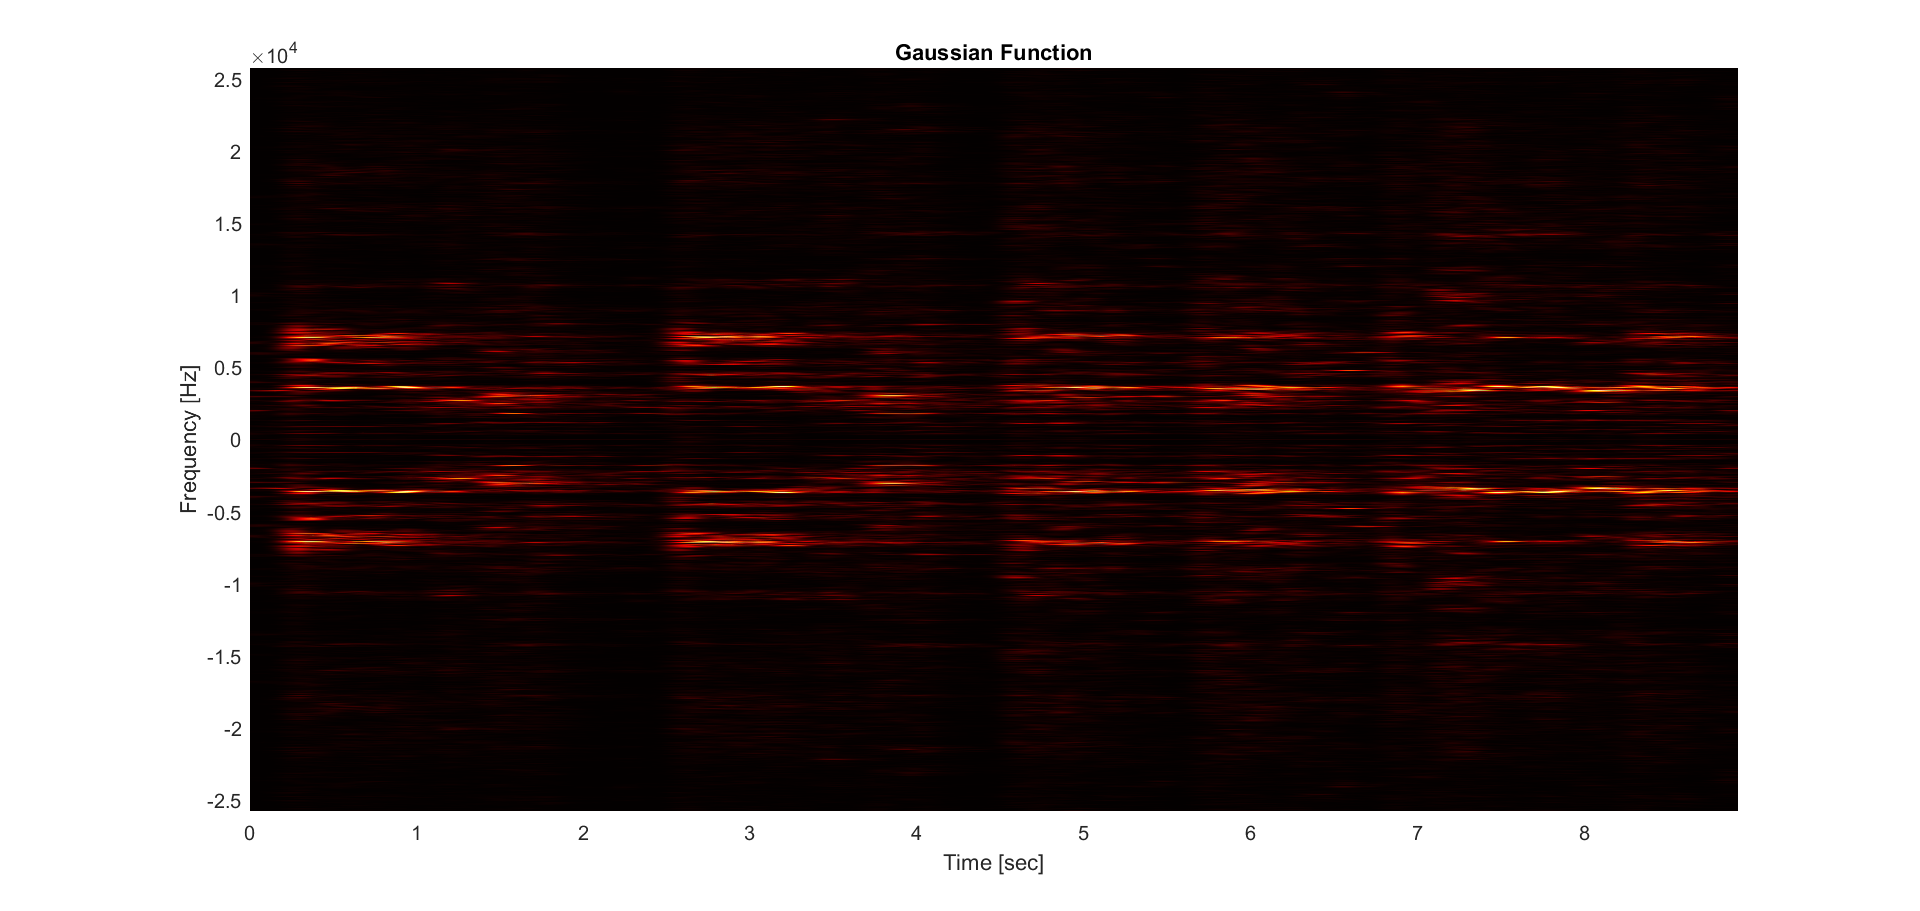
\includegraphics[width = 0.5\linewidth]{./Figures/oversampling001}}
\caption{Spectrograms show the effect of sliding parameter $\tau$ on the spectral and temporal resolution using Gaussian window function of FWHM $\approx 0.2$.}
\label{fig:sliding}
\end{figure}

The figure \ref{fig:scaling} shows the effect of undersampling and oversampling. For large $\tau$, the signal was undersampled as a result of which both frequency and temporal resolution deteriorated. Infact, nearly half of the signal was not used during course sampling. On the other hand, for very small $\tau$, we get great temporal and spectral resolution but at the expense of computation time. While the resolution did not change significantly when $\tau$ was changed from $0.05$ to $0.01$, the computation time increased by $6$ folds.

\subsection{Part II}
In this section, first the piano and recorder recordings of the song were tranformed into vectors (as shown in figure \ref{fig:recording}. Using sampling rates for each recordings, corresponding time vectors were calculated. A Gaussian sliding window was constructed with width (FWHM) $\approx 0.2$ sec. The sliding step was chosen to be $\Delta \tau = 0.05$ sec. A logarithmic spectrogram was generated to find principal frequencies that has highest magnitudes. Bright spots in zoomed logarithmic spectrograms correspond to principal frequencies while less bright spots indicate overtones. Using the music chart and the zoomed spectrogram of piano recording, the music score was found to be: \textbf{B A G A B B B A A A B B B B A G A B B B B A A B A G}.

By comparing spectrograms in the figure \ref{fig:zspectrogram}, we can see that piano generates excessive overtones than recorder. These overtones, which are interger multiples of principal frequencies, gives the piano music a rich sound (often known as timbre of the instrument).

\begin{figure}[!h]
\subfloat[Piano recording.]{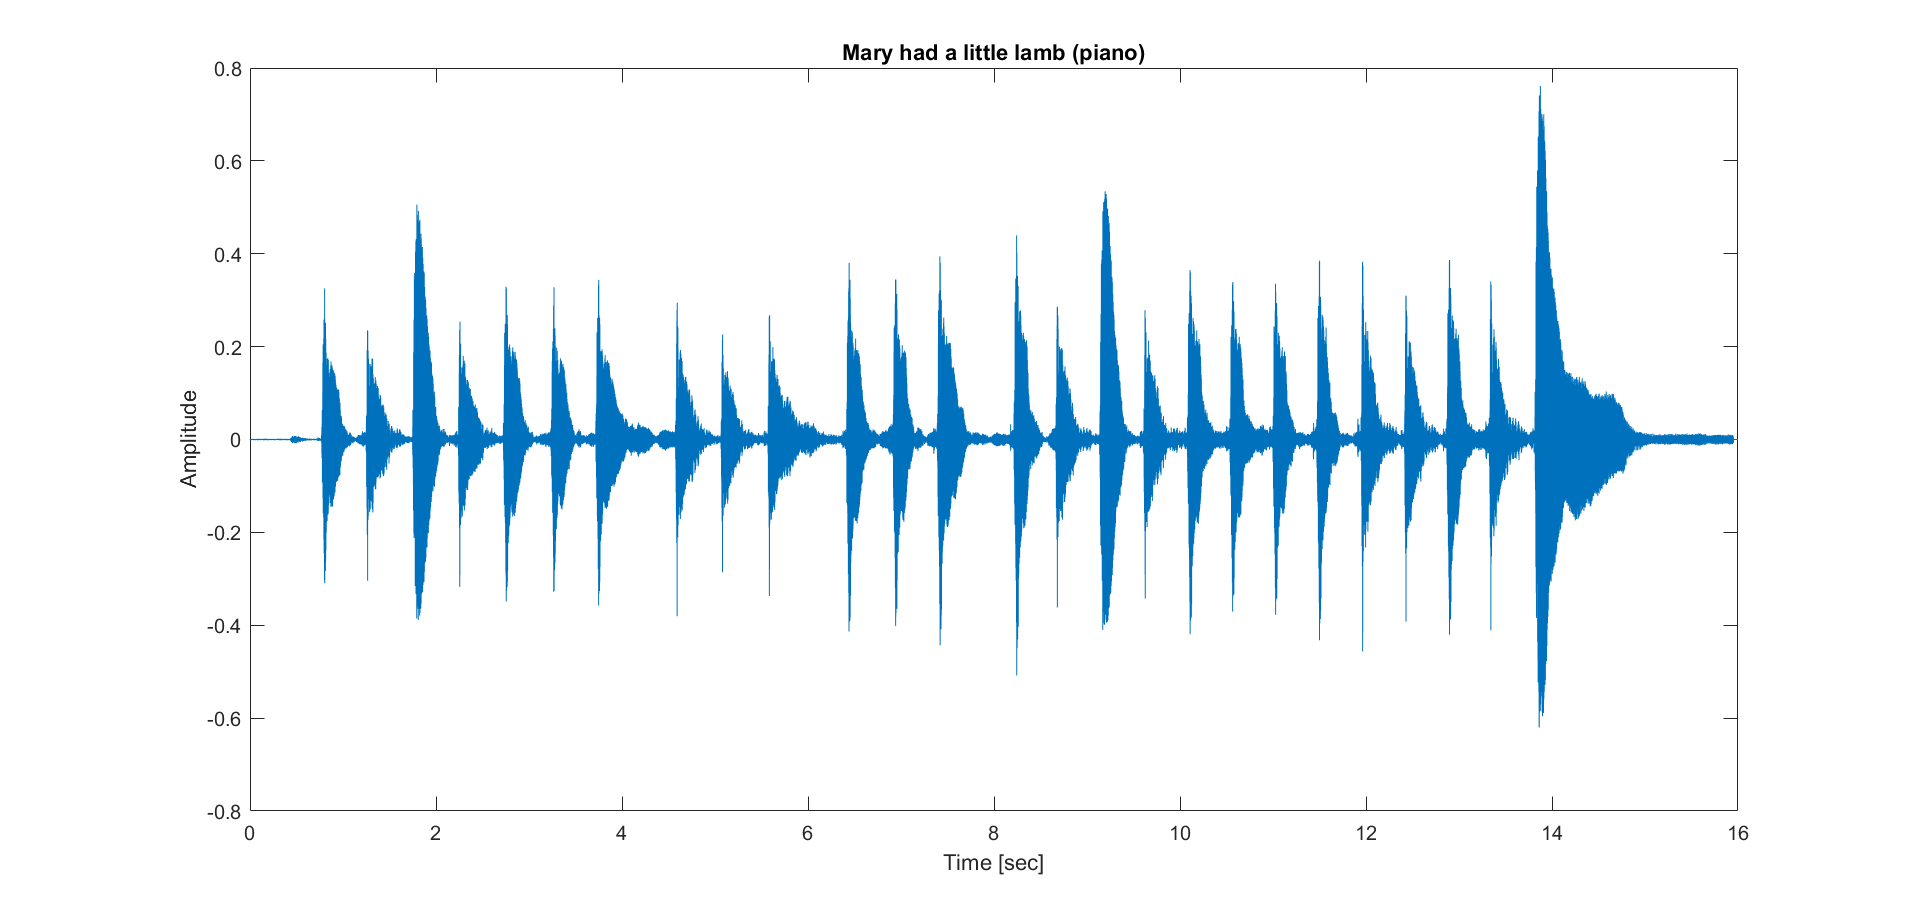
\includegraphics[width = 0.5\linewidth]{./Figures/piano}} 
\subfloat[Recorder recording.]{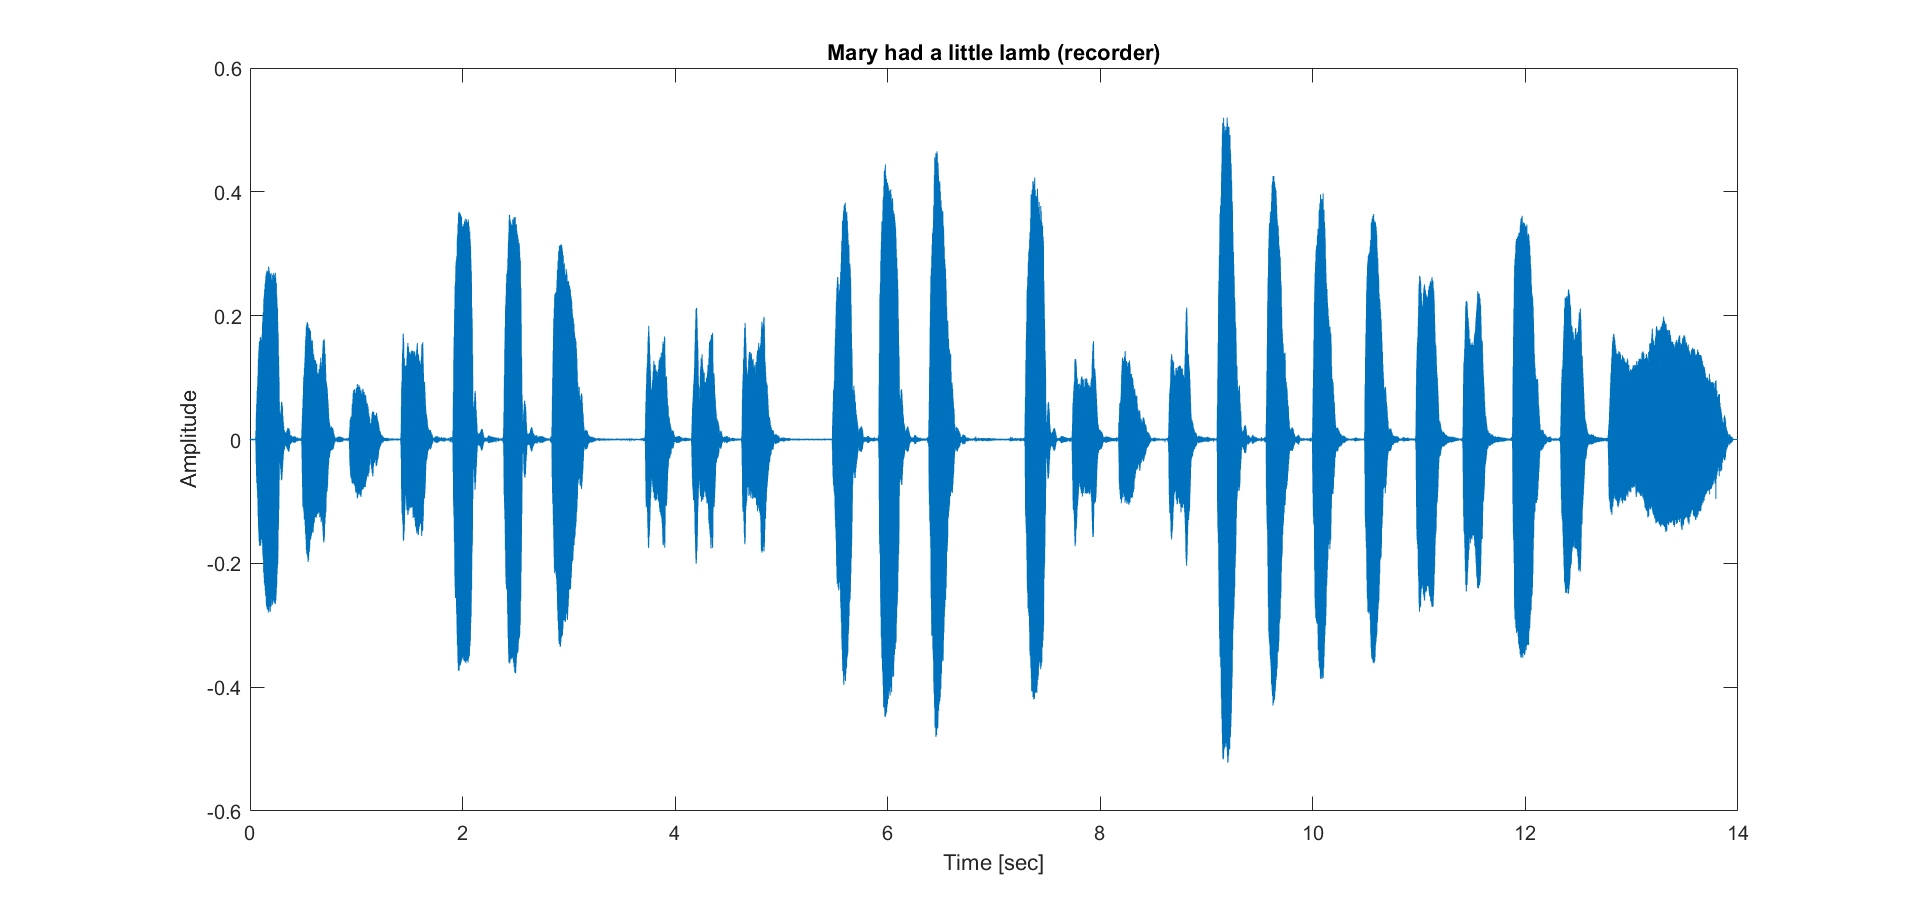
\includegraphics[width = 0.5\linewidth]{./Figures/recorder}}
\caption{Figure shows piano and recorder recordings of the song \textit{"Mary had a little lamb"}.}
\label{fig:recording}
\end{figure}

\begin{figure}[!h]
\subfloat[Zoomed logarithmic spectrogram of piano.]{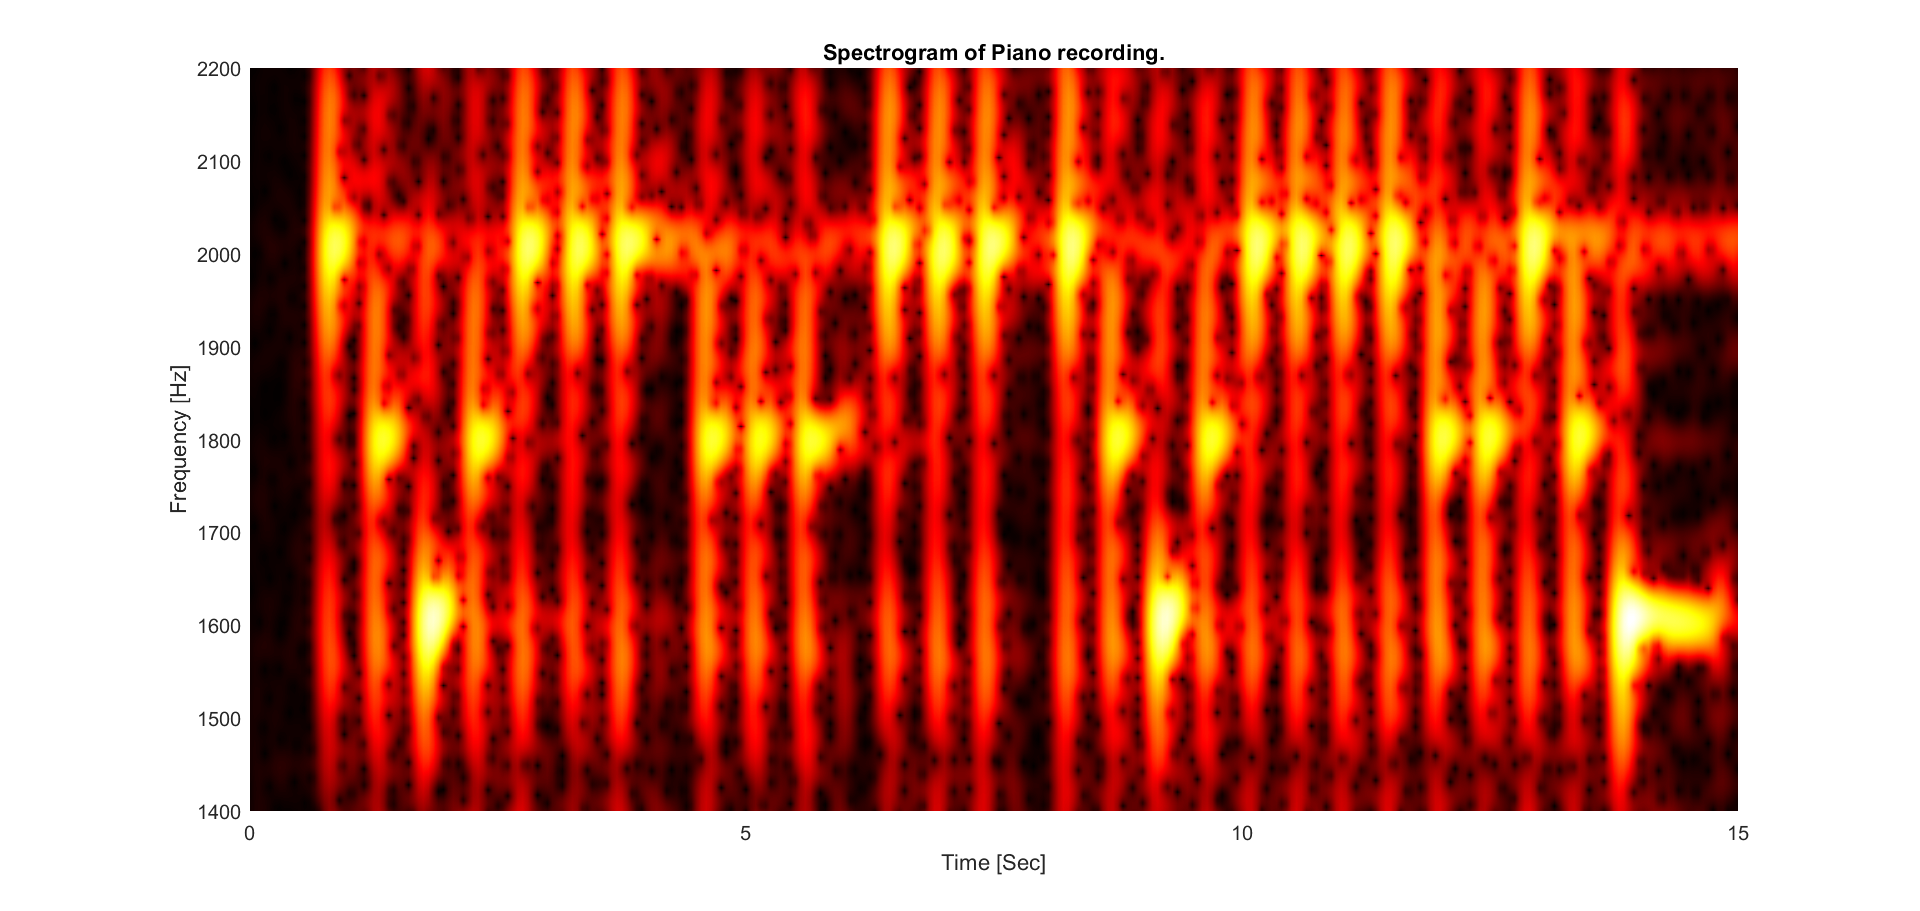
\includegraphics[width = 0.5\linewidth]{./Figures/zpiano}} 
\subfloat[Zoomed logarithmic spectrogram of recorder.]{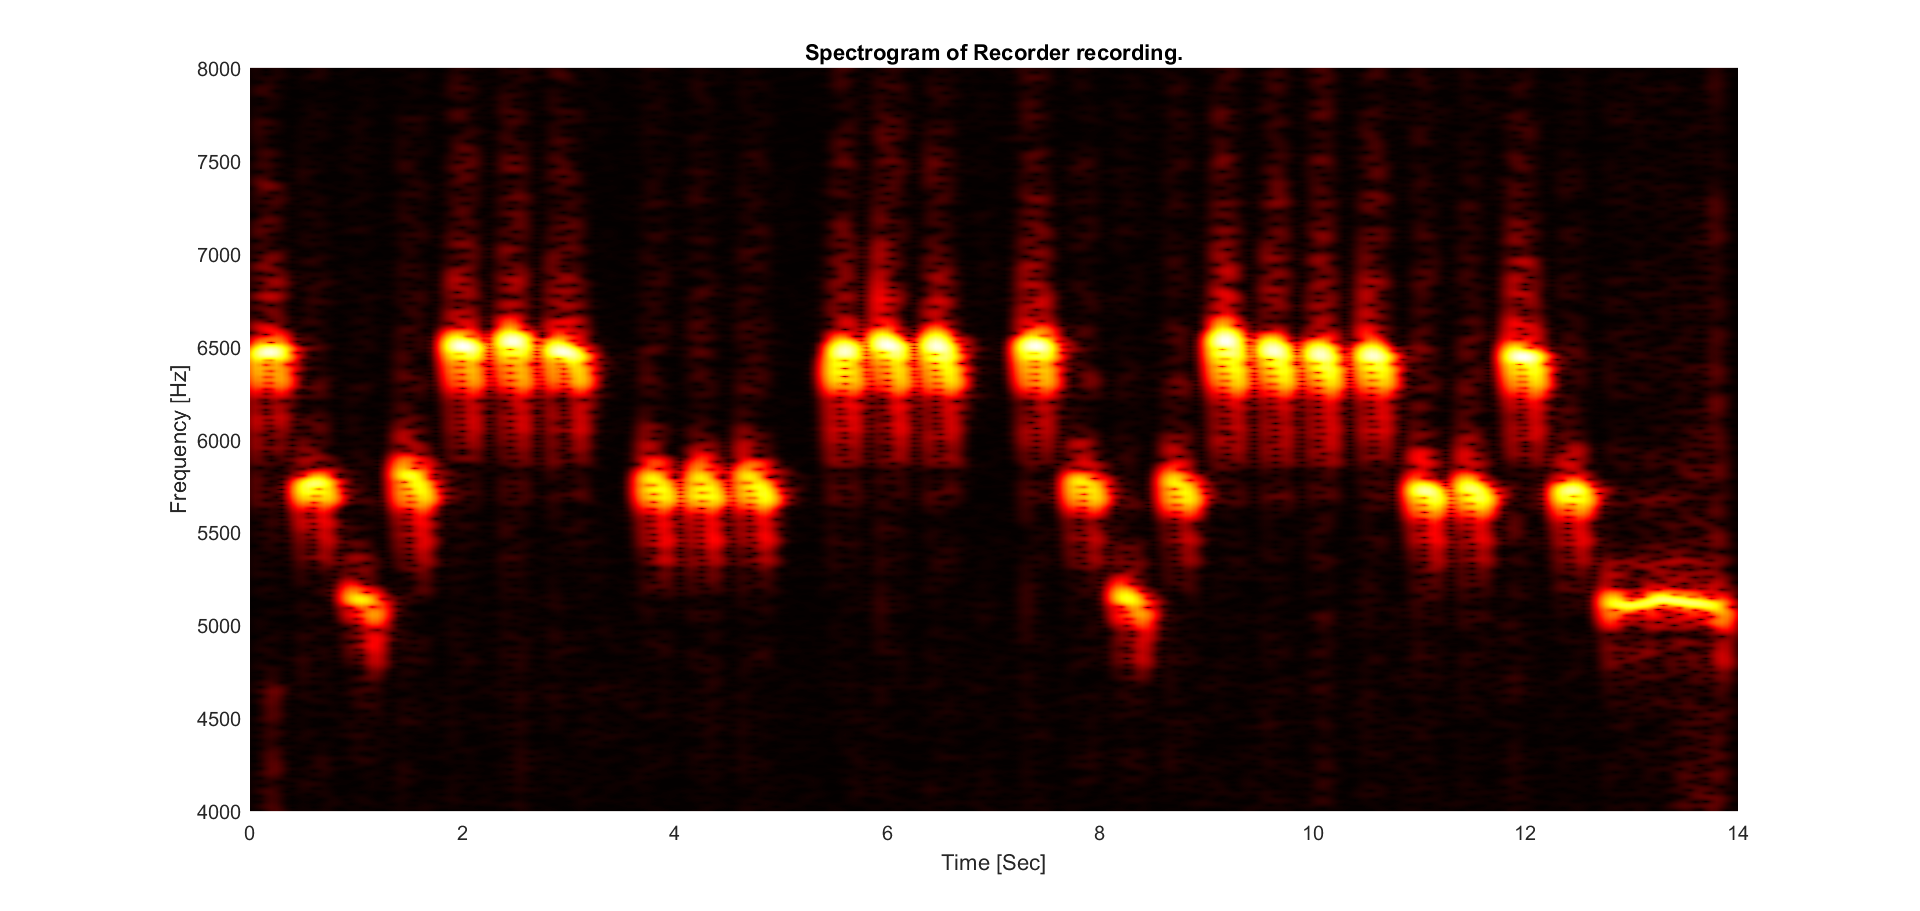
\includegraphics[width = 0.5\linewidth]{./Figures/zrecorder}}
\caption{Figure shows zoomed logarithmic spectrograms of piano and recorder recordings using Gaussian sliding window.}
\label{fig:zspectrogram}
\end{figure}

% Summary and Conclusions
\section{Summary and Conclusions}
In this paper, Gabor transform was analyzed using music recordings. In the first part, using Handel's Messiah recording, the effect of changing sliding and scaling parameters on the temporal and spectral resolution of spectrogram was studied. It was concluded that Gabor transform provides temporal resolution but at the expense of spectral resolution. The sliding window and its parameters should be chosen so that both temporal and spectral resolutions are maximized. For both data, it was found that the Gaussian sliding window of width $0.2$ with sliding time step of $0.05$ gave good resolutions. Spectrograms for $3$ different sliding window function (Gaussian, Mexican Hat and Shannon) was also analyzed. In the second part, music score of a piano recording was reproduced using Gabor tranform. By comparing spectrograms of recorder and piano recordings, it was found that the richness of sound in piano comes from overtones. Using the music sheet for piano, the music score was reproduced.

\pagebreak
% Appendices
\begin{appendices}

% MATLAB Functions
\section{MATLAB Functions}
Some important MATLAB functions used during the implementation.
\begin{itemize}
    \item \texttt{y = linspace(x1,x2,n)} returns a row vector of \texttt{n} evenly spaced points between \texttt{x1} and \texttt{x2}. 
    \item \texttt{ks = fftshift(k)} rearranges FT by shifting zero frequency component to the center of the array. Exchanges two halves of the array.
    \item \texttt{Y = fftn(X)} returns multidimensional Fourier transform of an N-D array using FFT algorithm
    \item \texttt{pcolor(X,Y,C)} specifies the x- and y-coordinates for the vertices. The size of C must match the size of the x-y coordinate grid. For example, if X and Y define an m-by-n grid, then C must be an m-by-n matrix.
    \item \texttt{colormap(map)} sets the colormap for the current figure to the colormap specified by map.
    \item \texttt{shading interp} varies the color in each line segment and face by interpolating the colormap index or true color value across the line or face.
\end{itemize}

\pagebreak
% MATLAB Codes

\section{MATLAB Code}
\href{https://github.com/cssubedi/AMATH-582}{The code is published on the github repository AMATH-582 under Gabor Transform directory.} \\

\textbf{MATLAB code for Part I of the assignment.}
\lstinputlisting[style=Matlab-editor]{GaborTransform.m}
\pagebreak
\textbf{MATLAB code for Part II of the assignment.}
\lstinputlisting[style=Matlab-editor]{Spectrogram.m}

%\begin{listing}[h]
%\inputminted{matlab}{example.m}
%\caption{Example code from external file.}
%\label{listing:examplecode}
%\end{listing}

\end{appendices}

\end{document}
